\documentclass[12pt]{article}
\usepackage{graphicx}
\usepackage{multirow}
\usepackage{fullpage}
\usepackage{times}
\usepackage{tipa}
\usepackage[normalem]{ulem}
\setlength\parindent{0pt}
\setlength\parskip{12pt}

\usepackage{amsmath}
\usepackage{amssymb}
\usepackage[utf8]{inputenc}

\newcommand{\auth}{\text{auth}}
\newcommand{\paperby}{\text{paperBy}}
\newcommand{\reviewofby}{\text{reviewOfBy}}
\newcommand{\bool}{\text{bool}}
\newcommand{\rev}{\text{rev}}

\begin{document}

{\sffamily
\begin{tabular}{ll}
\multirow{3}{*}{\includegraphics[width=1in]{ach.png}}\\
& \textbf{\Huge{SIGBOVIK 2020}} \\ &\\
& \LARGE{Message from the Organizing Committee} \\
&\\
\hline
\end{tabular}}
\vspace{2em}
\thispagestyle{empty}

For generality’s sake, we have templatized the message of the organizing committee. The actual message may be produced by running the TeX command at the end.

\begin{verbatim}
\newcommand{\Message2020}[3]{
% TODO: generalize ordinal indicators
\end{verbatim}
Friends, family, colleagues, acquaintances for whom we have not yet overcome the activation energy to engage with regularly, and strangers doomed to the same fate: The Association of Computational Heresy welcomes you to the \#1\textsuperscript{th} annual meeting of the Special Interest Group on Harry Q\#2 Bovik in celebration of Bovik’s \#3\textsuperscript{th} birthday. In lieu of data about the submission and review process this year, we encourage you to ponder the perils of empiricism as well as our innovations in the publishing process: most notably, triple-blind peer review. In plain English, we have the following definition.\\

\textbf{triple-blind peer review} /\textipa{\textprimstress tr\textsci pl-bla\textsci nd pi\textlengthmark r r\textsci\textprimstress vju\textlengthmark}/ \emph{noun}
\begin{enumerate}
\item Scholarly peer review that minimizes bias by concealing not only the identities of the authors and reviewers from each other, but also by concealing the papers from the reviewers. Compare: single- and double-blind peer review.
\end{enumerate}
However, let us undertake some performative formalization. Given a set of names of authors $(\auth)$ and reviewers ($\rev$), we consider the role of author and reviewer as, under the Curry-Howard correspondence, proofs of the following higher-order linear logic propositions/processes conforming to the following protocols.
\begin{align*}
&\vdash P::(c:\exists_{a:\auth,p:\paperby(a)}\forall_{r:\rev}\reviewofby(p, r)\multimap\bool)\\
&\vdash Q::(d:\forall_{a:\auth,p:\paperby(a)}\exists_{r:\rev}\reviewofby(p, r))
\end{align*}
Under duality, it is clear that communication between $P$ and $Q$ is sound. Then, each level of blindness (single to triple) is achieved by successively abstracting the definition of $\rev$ for $P$ then $\auth$ and $\paperby$ for $Q$ respectively; we refer to the work of Harper and Lillibridge \cite{harper+:sharing} on translucent sums to achieve this. Higher-order notions of blind review require a stronger metatheory like a linear temporal-linear logical framework (that’s TWO linears!); we encourage future work to investigate this idea.
Now that the general chair has redeemed himself for not submitting a paper this year, we would like to thank our authors and reviewers for their phenomenal work and for adjusting to the new review process as well as the continuous effort of volunteers who have made this year’s conference possible, which include but are not limited to: Chris Yu for the cover art, Catherine Copetas for managing our finances and other administrative concerns, and Ryan Kavanagh for organising the organisers. Moreover, the program chair also thanks Rose Bohrer and Stefan Muller for further advice. Lastly, we would like to thank Sol Boucher for assembling the proceedings as well as Jenny Lin and Siva Somayyajula for never working in various capacities (see figure \ref{fig:never}).
\begin{figure}
\centering
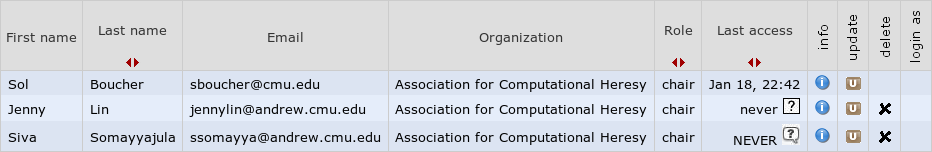
\includegraphics[width=\textwidth]{never.png}
\caption{never say NEVER}
\label{fig:never}
\end{figure}
\begin{flushright}
The SIGBOVIK 2020 Organising Committee\\
Pittsburgh, PA

Jenny Lin (easy chair)\\
Siva Somayyajula (generalized hard-ass chair)\\
Sol Boucher (fold-out couch)\\
Rose Bohrer (reclining chair)\\
Ryan Kavanagh (rockin' chair)\\
Chris Yu (swivel chair)\\
Stefan Muller (ergonomic office chair)
\end{flushright}
\begin{verbatim}
}
\Message2020{14}{uarantine}{$2^6$}
\end{verbatim}

\bibliographystyle{acm}
\bibliography{msgrefs}
\thispagestyle{empty}


\end{document}
